%\documentclass[a5paper,headsepline,titlepage,11pt,nnormalheadings,DIVcalc]{scrbook}
\documentclass[a5paper,headsepline,titlepage,11pt,nnormalheadings,DIVcalc]{book}
\usepackage[a5paper,backref]{hyperref}
\usepackage[papersize={165mm,215mm},twoside,bindingoffset=0.5cm,hmargin={2cm,2cm},
				vmargin={2cm,2cm},footskip=1.1cm,driver=dvipdfm]{geometry}
%\usepackage[papersize={148mm,215mm},twoside,bindingoffset=0.5cm,hmargin={2cm,2cm},
%				vmargin={2cm,2cm},driver=dvipdfm]{geometry}
%\usepackage{palatino}
\usepackage{graphicx}
\usepackage{wrapfig}
\usepackage[bahasa]{babel}
\usepackage{fancyhdr}
\usepackage{longtable}
\usepackage{hhline,multirow}
\usepackage{pst-node}

%\setlength{\voffset}{0.5in}
%\setlength{\oddsidemargin}{28pt}
%\setlength{\evensidemargin}{0pt}
\renewcommand{\footrulewidth}{0.5pt}
\lhead[\fancyplain{}{\thepage}]%
      {\fancyplain{}{~}}
\rhead[\fancyplain{}{~}]%
      {\fancyplain{}{\thepage}}
\pagestyle{fancy}
\lfoot[\emph{Informasi 2010}]{}
\rfoot[]{\emph{Lingkungan St Petrus Maguwo}}
\cfoot{}

\newcommand{\BU}[1]{\begin{itemize} \item[U:] #1 \end{itemize}}
\newcommand{\BI}[1]{\begin{itemize} \item[I:] #1 \end{itemize}}
\newcommand{\BP}[1]{\begin{itemize} \item[P:] #1 \end{itemize}}
\title{Informasi Lingkungan St. Petrus}
\author{Wilayah Yohanes De Britto \\Stasi Maguwo \\Paroki Kalasan}
\date{2010}
\hyphenation{a-kan}
\hyphenation{ba-gi-mu}
\hyphenation{ber-a-da}
\hyphenation{ber-du-a}
\hyphenation{be-ri-kan}
\hyphenation{ber-ka-ta}
\hyphenation{ber-nya-nyi}
\hyphenation{ber-sa-ma}

\hyphenation{dah-syat}
\hyphenation{DA-RAH-KU}
\hyphenation{da-tang}
\hyphenation{di-ka-ta-kan}
\hyphenation{di-pim-pin}
\hyphenation{di-se-rah-kan}
\hyphenation{di-tum-pah-kan}

\hyphenation{Eng-kau}
\hyphenation{ha-dap-an}
\hyphenation{han-tar-kan-lah}
\hyphenation{ha-rap-an}

\hyphenation{ja-lan}
\hyphenation{ja-ngan-lah}

\hyphenation{ka-nak}
\hyphenation{ka-re-na}
\hyphenation{kau-lim-pah-kan}
\hyphenation{Kau-cip-ta-kan}
\hyphenation{ke-bang-kit-an-Nya}
\hyphenation{ke-da-tang-an}
\hyphenation{ke-da-tang-an-Nya}
\hyphenation{ke-dua}
\hyphenation{ke-na-ik-kan-nya}
\hyphenation{ke-pa-daMu}
\hyphenation{ke-ra-him-an}
\hyphenation{ke-se-jah-te-ra-an-mu}
\hyphenation{ko-men-tar}

\hyphenation{la-ma-nya}
\hyphenation{lim-pah-kan}

\hyphenation{ma-nu-sia}
\hyphenation{me-nga-da-kan}
\hyphenation{me-ngan-dung-lah}
\hyphenation{me-ngu-kuh-kan}
\hyphenation{me-la-lui}
\hyphenation{me-lim-pah-kan}
\hyphenation{me-lu-hur-kan}
\hyphenation{me-me-cah-me-cah-kan}
\hyphenation{mem-per-sem-bah-kan}
\hyphenation{me-nan-da-ta-ngan-i}
\hyphenation{men-cin-tai}
\hyphenation{meng-a-lir-kan}
\hyphenation{me-nga-sihi}
\hyphenation{me-nge-lu-ar-kan}
\hyphenation{meng-u-cap-kan}
\hyphenation{meng-ung-kap-kan}
\hyphenation{me-num-buh-kan}
\hyphenation{me-nya-ta-kan}
\hyphenation{me-nye-la-mat-kan}
\hyphenation{me-nye-rah-kan}
\hyphenation{me-nye-rah-kanNya}
\hyphenation{me-ra-ya-kan}

\hyphenation{o-rang}
\hyphenation{o-rang-o-rang}

\hyphenation{pa-sang-kan-lah}
\hyphenation{pa-tut}
\hyphenation{pe-ne-ri-ma-an}
\hyphenation{pe-ngam-pun-an}
\hyphenation{Pe-ngan-ta-ra}
\hyphenation{peng-hi-bur-an}
\hyphenation{per-bu-at-an-nya}
\hyphenation{per-ka-ta-an}
\hyphenation{per-ka-win-an}
\hyphenation{per-ni-kah-an}
\hyphenation{per-se-ku-tu-an}
\hyphenation{per-sem-bah-an}
\hyphenation{rom-bong-an}

\hyphenation{se-la-ma}
\hyphenation{se-ka-li-an}
\hyphenation{se-pan-jang}
\hyphenation{se-ra-ya}
\hyphenation{Su-dar-yan-to}

\hyphenation{te-ta-pi}
\hyphenation{ta-ngan-Mu}
\hyphenation{Tu-han}
\hyphenation{tu-lang}
\hyphenation{tu-lang-tu-lang}

\hyphenation{u-mat-Mu}
\hyphenation{wa-kil}

\hyphenation{ba-gi-mu}
\hyphenation{di-se-rah-kan}
\hyphenation{me-la-lui}
\hyphenation{ka-nak}
\hyphenation{ka-re-na}
\hyphenation{ber-ka-ta}
\hyphenation{te-ta-pi}
\hyphenation{per-ka-win-an}
\hyphenation{pa-tut}
\hyphenation{me-lu-hur-kan}
\hyphenation{ber-nya-nyi}
\hyphenation{di-tum-pah-kan}
\hyphenation{pe-ngam-pun-an}
\hyphenation{ber-a-da}
\hyphenation{kau-lim-pah-kan}
\hyphenation{ke-bang-kit-an-Nya}
\hyphenation{per-ka-ta-an}
\hyphenation{pa-sang-kan-lah}
\hyphenation{DA-RAH-KU}
\hyphenation{ke-na-ik-kan-nya}
\hyphenation{per-sem-bah-an}
\hyphenation{per-se-ku-tu-an}


\renewcommand*\thesection{\arabic{section}.}
\setlength{\parindent}{0mm} 

\begin{document}
\thispagestyle{empty}
%\maketitle
\newsavebox\IBox
%\sbox\IBox{\includegraphics[scale=0.4]{Saint-Peter-Apostle-e.eps}}

%% \psset{unit=1in}
%% \begin{pspicture}(4in,6.0in)
%% % set up the fonts we use
%% \DeclareFixedFont{\PT}{T1}{ppl}{b}{it}{0.4in}
%% \DeclareFixedFont{\PTsmall}{T1}{ppl}{b}{it}{0.3in}
%% \DeclareFixedFont{\PTsmallest}{T1}{ppl}{b}{it}{0.2in}
%% \DeclareFixedFont{\PTtext}{T1}{ppl}{b}{it}{11pt}
%% \DeclareFixedFont{\Logo}{T1}{pbk}{m}{n}{0.2in}
%% % place the front cover picture
%% \rput[cb](2.3,2.5){\usebox\IBox}
%% % put the text on the front cover
%% \rput[cb](2.5,5.3){\PT {Informasi}}
%% \rput[cb](2.5,4.8){\PT {Lingkungan St. Petrus}}
%% \rput[cb](2.5,0.6){\PTsmallest {Wilayah Yohanes de Britto}}
%% \rput[cb](2.5,0.3){\PTsmallest {Stasi Maguwo}}
%% \rput[cb](2.5,0.0){\PTsmallest {Paroki Marganingsih Kalasan }}
%% 
%% %\rput[cb](3,-1){\PTsmallest {\namagereja}} 
%% 
%% \end{pspicture}
%\tableofcontents 

\setlength{\parskip}{2mm}
\section*{Sejarah singkat Lingkungan St Petrus}
Lingkungan Santo Petrus yang ada sekarang ini (2010) sudah melewatai banyak liku-liku. Pada awalnya, yauitu tahun 1984, bernama Kring Santo Petrus yang meliputi dusun Nanggulan, Kopenrejo, Gondangan, Setan, Dewan, Kalongan,  dan Kembang. Kepengurusan periode awal ini diketuai oleh Ig. Mulyono yang diberkati oleh Rm Y. Suyadi, Pr, romo paroki Kalasan saat itu. Kepengurusan ini berakhir pada tahun 1987.

Periode berikutnya 1987-1990 Kring St Petrus memiliki umat sebanyak 159 warga dalam 53 keluarga dan sebagai ketua kring adalah Th Sukamto. 
%Peristiwa penting dalam periode ini adalah peresmian Gereja Bunda Maria oleh Uskup Agung Mgr. Y. Darmoatmojo SJ pada 2 Juni 1988. Selain itu pada tanggal 10 Oktober 1989 ada kunjungan Sri Paus Yohanes Paulus II di Yogyakarta. Gereja Bunda Maria mendapat kenang-kenangan berupa karpet merah sepanjang 25 m yang pernah dilalui oleh Sri Paus saat misa akbar di Adisucipto.
Pada penyerahan kepengurusan dari periode sebelumnya, H. Siswanto sebagai ketua lingkungan periode 1990-1993 menerima data jumlah umat lingkungan St Petrus sudah berkembang menjadi 71 keluarga yang terdiri atas 213 warga. Perubahan dari kring menjadi lingkungan sesuai dengan perubahan Wilayah Maguwo menjadi Stasi Maguwo pada tahun 1990. 
%Saat kepengurusan H. Siswanto ini terjadi mutasi 4 keluarga dengan 12 warga masuk dan 1 keluarga dengan 3 warga keluar. 
Mengingat wilayah St Petrus yang luas maka sesuai dengan kesepakatan dilakukan pemekaran menjadi 2 lingkungan yaitu St Petrus dan St Paulus. Lingkungan St Petrus meliputi Kembang, Nanggulan, Gondangan, Tajem, Setan, Karang Nongko, Sopalan. Lingkungan Paulus meliputi Rejoinangun, Dewan, Kalongan, Corongan.

Periode berikutnya 1993-1995 umat lingkungan mencapai 58 keluarga terdiri atas 223 warga dengan ketua T. Sukijo. Periode 1996-2001 ketua lingkungan dijabat oleh V. Sukiyanto dengan umat sejumlah 256 warga dalam 69 keluarga. Saat ketua dijabat oleh Y. Samin (2002-2004) umat berkembang menjadi 76 keluarga dengan 270 warga.

Wilayah Lingkungan St Petrus masih dirasa terlalu luas maka pada tahun 2006 saat kepengurusan FX Radjijo (2005-2007) dilakukan pemekaran lagi menjadi 2 lingkungan yaitu St Petrus dan St Fransiskus Asisi. Kedua wilayah dibatasi oleh {\it ring road}. 

Periode transisi 2006-2007 lingkungan St Petrus diketuai oleh Y.Z. Budiman S dengan umat sebanyak 162 dalam 48 keluarga. Saat ini lingkungan St Petrus mempunyai umat sebanyak 187 dalam 63 keluarga dan diketuai oleh V. Agung Danan Jaya.
 
\chapter*{Informasi Umat}

\section[Pengurus]{Pengurus lingkungan}

\subsection{Periode 2014 -- 2016}

%\footnotesize 
\begin{center}
SUSUNAN PENGURUS LINGKUNGAN SANTA THERESIA 
\par
PERODE TAHUN 2014 -- 2016
\end{center}

\begin{longtable}{p{0.5cm}p{4cm}p{5cm}p{4cm}}
\multicolumn{2}{l}{Ketua I}&Antonius Supriyana &+6285 865 355 895\\
\multicolumn{2}{l}{Ketua II}&FX. Sularto &+6281 314 190 698\\
\multicolumn{2}{l}{Sekretaris I}&Anastasi Bare &+6285 643 173 281\\
\multicolumn{2}{l}{Sekretaris II}&FX. Ari Wibowo Sudaryanto&+6285 8633 5678\\
\multicolumn{2}{l}{Bendahara I}&Theresia Prima Ari Setiyani&+6285 6288 6539\\
\multicolumn{2}{l}{Bendahara II}&Agnes Sukarmi&+6281 328 795 814\\

\setcounter{nourut}{0}\\
\multicolumn{2}{l}{\textit{\textbf{Tim Kerja Liturgi}}}&&\\
&Koordinator&Yohanes Suyanto &+6285 6286 9037\\
\nexturut&Misa/Peribadatan/Doa Lingk &M.Th. Nanik Ismarjati&+6281 5686 1272\\
\nexturut&Koor&Maria Sode Muda&+6281 392 842 606\\
&&Andreas Keso Muda&+6281 328 692 102\\

\setcounter{nourut}{0}\\
\multicolumn{2}{l}{\textit{\textbf{Tim Kerja Pewartaan}}}&Neo Suradi&+6281 578 115 615\\

\setcounter{nourut}{0}\\
\multicolumn{2}{l}{\textit{\textbf{Tim Kerja Kemasyarakatan}}}&&\\
&Koordinator&Cornelius Triyono &+6281 578 179 267\\
\nexturut&Tabungan Cinta Kasih (TCK)&Kristina Tri Tutwuri &+6281 2275 2803\\
\nexturut&Prolenan&A. Sri Supriyati &+6281 328 450 101\\
\nexturut&Pangruktilaya&Th. Suci Wahyuningsih&+6281 5792 7488 \\
&&M. Th. Nanik Ismarjati&+6281 5686 1272\\
\nexturut&PSE&A. Sri Supriyati&+6281 328 450 101\\
\nexturut&Majalah Paroki/Lingkungan&OMK Lingkungan&\\

\setcounter{nourut}{0}\\
\multicolumn{2}{l}{\textit{\textbf{Tim Kerja Paguyuban}}}&&\\
&Koordinator&Ketua II&\\
\nexturut&Pag. Ibu-ibu Lingkungan&A. Hedwig Djuwarni&+6281 578 898 484\\
&&M.Goretti Budi Hartati&+6285 878 241 474\\
\nexturut&Pag. OMK Lingkungan&Stefanus Pratama Krisna Bayu Aji&\\
\nexturut&Pendamping OMK Lingk.&Neo Suradi&+6281 578 115 615\\

\setcounter{nourut}{0}\\
\multicolumn{2}{l}{\textit{\textbf{Tim Kerja Rumah Tangga}}}&&\\
\nexturut&Paramenta&Yohanes Suyanto&+6285 6286 9037\\
\nexturut&Tata Bunga&C. Prihatiningtyas S.&+6287 838 452 319\\
&&M.M.S.U.Chrissumiwi&+6281 392 301 293\\


\setcounter{nourut}{0}\\
\multicolumn{2}{l}{\textit{\textbf{Tim Kerja Humas}}}&&\\
&Koordinator&Sekretaris I&\\
\nexturut&Pugeran Utara &Kristina Tri Tutwuri &+6281 2275 2803\\
\nexturut&Pugeran Selatan&Lusia Titisari&+6283 867 812 334\\
\nexturut&Sombomerten+Pugeran Timur&Herminigilda A. Wulandari&+6287 843 023 654\\
\end{longtable}

\subsection{Periode 2017 -- 2019}

\begin{center}
	SUSUNAN PENGURUS LINGKUNGAN SANTA THERESIA 
	\par
	PERIODE TAHUN 2017 -- 2019
\end{center}
%\footnotesize 
\begin{longtable}{p{0.5cm}p{4cm}p{5cm}p{4cm}}
	\multicolumn{2}{l}{Ketua I}&Antonius Supriyana &+6285 865 355 895\\
	\multicolumn{2}{l}{Ketua II}&FX. Sularto &+6281 314 190 698\\
	\multicolumn{2}{l}{Sekretaris I}&M.M.S.U. Chrissumiwi &+6281 392 301 293\\
	\multicolumn{2}{l}{Bendahara I}&Theresia Prima Ari Setiyani&+6285 6288 6539\\
	\multicolumn{2}{l}{Bendahara II}&Agnes Sukarmi&+6281 328 795 814\\
	
	\setcounter{nourut}{0}\\
	\multicolumn{2}{l}{\textit{\textbf{Tim Kerja Liturgi}}}&&\\
	&Koordinator&Yohanes Suyanto &+6285 6286 9037\\
	\nexturut&Misa/Peribadatan/Doa Lingkungan &M.Th. Nanik Ismarjati&+6281 5686 1272\\
	\nexturut&Koor&Maria Sode Muda&+6281 392 842 606\\
	&&Valentina Isti Rudati&+6281 328 692 102\\
	
	\setcounter{nourut}{0}\\
	\multicolumn{2}{l}{\textit{\textbf{Tim Kerja Pewartaan}}}&Neo Suradi&+6281 578 115 615\\
	
	\setcounter{nourut}{0}\\
	\multicolumn{2}{l}{\textit{\textbf{Tim Kerja Kemasyarakatan}}}&&\\
	&Koordinator&Cornelius Triyono &+6281 578 179 267\\
	\nexturut&Tabungan Cinta Kasih (TCK)&Kristina Tri Tutwuri &+6281 2275 2803\\
	\nexturut&Prolenan&Roselina Zeli Puspitasari &\\
	\nexturut&Pangruktilaya&M. Th. Nanik Ismarjati&+6281 5686 1272\\
	&&C. Prihatiningtyas&+6287 838 4523\\
	\nexturut&PSE&Yohanes Sudarmadi&+6281 328 450 101\\
	\nexturut&Majalah Paroki/Lingkungan&OMK Lingkungan&\\
	
	\setcounter{nourut}{0}\\
	\multicolumn{2}{l}{\textit{\textbf{Bidang Paguyuban}}}&&\\
	&Koordinator&Aloysius Heru Pratomo&+6281 328 259 725\\
	\nexturut&Pag. Ibu-ibu Lingkungan&Anastasia Sri Supriyati&+62 813 2845 0101\\
	\nexturut&Pag. OMK Lingkungan&Maria Regina Tri Marieska&+62 813 9205 4103\\
	\nexturut&Pendamping OMK Lingk.&Andreas Keso Muda&+6281 328 692 102\\
	
	\setcounter{nourut}{0}\\
	\multicolumn{2}{l}{\textit{\textbf{Bidang Rumah Tangga}}}&&\\
	&Koordinator&Yohanes Djoko Marsito&+62 858 2013 3321\\
	\nexturut&Paramenta&Yohanes Suyanto&+6285 6286 9037\\
	\nexturut&Tata Bunga&C. Prihatiningtyas S.&+6287 838 452 319\\
	&&M.M.S.U.Chrissumiwi&+6281 392 301 293\\
	
	
	\setcounter{nourut}{0}\\
	\multicolumn{2}{l}{\textit{\textbf{Litbang dan Data umat}}}&&\\
	&&Andreas Keso Muda&\\
	&&Yohanes Suyanto&\\
\end{longtable}


\begin{longtable}{|m{5mm}|m{45mm}|m{20mm}|m{20mm}|m{5mm}|m{25mm}|m{20mm}|} 
	\hline  
	\multicolumn{1}{|c|}{\multirow{2}{*}{\textbf{No}}} & \multicolumn{1}{|c|}{\multirow{2}{*}{\textbf{Nama}}} 
	& \multicolumn{2}{|c|}{\textbf{Lahir}} 
	& \multicolumn{1}{|c|}{\multirow{2}{*}{\textbf{L/P}}}
	&\multicolumn{2}{|c|}{\textbf{Baptis}}  \\ \cline{3-4}\cline{6-7}
	&
	&\multicolumn{1}{|c|}{\textbf{Tempat}} & \multicolumn{1}{|c|}{\textbf{tanggal}} 
	&
	&\multicolumn{1}{|c|}{\textbf{Tempat}} & \multicolumn{1}{|c|}{\textbf{tanggal}} \\ 
	\hline \hline  \endfirsthead 
	\hline  
	\multicolumn{1}{|c|}{\multirow{2}{*}{\textbf{No}}} & \multicolumn{1}{|c|}{\multirow{2}{*}{\textbf{Nama}}} 
	& \multicolumn{2}{|c|}{\textbf{Lahir}} & 
	\multicolumn{1}{|c|}{\multirow{2}{*}{\textbf{L/P}}}
	& \multicolumn{2}{|c|}{\textbf{Baptis}}  \\ \cline{3-4}\cline{6-7}
	&
	&\multicolumn{1}{|c|}{\textbf{Tempat}} & \multicolumn{1}{|c|}{\textbf{tanggal}} 
	&
	&\multicolumn{1}{|c|}{\textbf{Tempat}} & \multicolumn{1}{|c|}{\textbf{tanggal}} \\ 
	\hline \hline \endhead \endfoot
	1&Banarudin, Thomas&Gandekan Lor&1966-12-31&L&Marganingsih Kalasan&1997-03-25\\ \hline 
	2&Sode Muda, Maria&Flores&1974-03-25&P&Flores&1974-05-19\\ \hline 
	3&Titisari, Lusia&Sleman&1997-06-28&P&Marganingsih Kalasan&1997-12-05\\ \hline 
	4&Keso Muda, Andreas&Flores&1957-11-13&L&Lewotobi Flores&1957-12-10\\ \hline 
	5&Sukarmi, Agnes&Musi Rawas Sumatera Selatan&1962-01-05&P&Tugumulyo&1966-09-01\\ \hline 
	6&Amarylis Illona Muda, Maria&Musi Rawas Sumatera Selatan&1987-12-30&P&Tugumulyo&1988-07-19\\ \hline 
	7&Sode Muda Valentia, Eleonora&Yogyakarta&1996-11-09&P&Marganingsih Kalasan&1997-01-03\\ \hline 
	8&Aloysius Lamakey&Flores&1948-06-07&L&Flores&0000-00-00\\ \hline 
	9&Chatarina Sukarmi&Nganjuk&1956-05-08&P&Gombong&1978-03-25\\ \hline 
	10&Lamakey Maria Anastasia Bare&Yogyakarta&1985-03-04&P&Kotabaru Yogyakarta&1985-03-13\\ \hline 
	11&Mardi Susanti, Agustina&Yogyakarta&1946-05-16&P&Kidulloji&0000-00-00\\ \hline 
	12&Nanik Ismarjati, Maria Theresia&Yogyakarta&1962-07-20&P&Kidulloji&1969-12-08\\ \hline 
	13&Temon Siswo Utomo, Margaretha&Bantul&1932-12-31&P&Pugeran&0000-00-00\\ \hline 
	14&Sandi Ignatius&Klaten&1942-02-25&L&Wedi Klaten&1964-03-28\\ \hline 
	15&Tri Susilowati, Caecilia&Yogyakarta&1952-09-21&P&Kemetiran&1952-11-22\\ \hline 
	16&Iglia Lucya, Paulina&Bantul&1995-11-06&P&Marganingsih Kalasan&2012-04-07\\ \hline 
	17&Sunaryo Prononagoro Kra, Yohanes Pemandi&Solo&1945-09-18&L&Sdh&0000-00-00\\ \hline 
	18&Setya Prihatiningtyas, Chatarina&Klaten&1977-08-07&P&Surabaya&0000-00-00\\ \hline 
	19&Apriliana Wulandari, Herminigilda&Sleman&2002-04-13&P&Marganingsih Kalasan&2002-07-05\\ \hline 
	20&Lintang Novianti, Maria&Sleman&2008-11-02&P&Marganingsih Kalasan&2008-12-05\\ \hline 
	21&Sudarmadi, Yohanes&Yogyakarta&1948-01-23&L&Kotabaru&1970-05-24\\ \hline 
	22&Djuwarni Anastasia Hedwig&Yogyakarta&1952-02-01&P&Kotabaru&1969-12-13\\ \hline 
	23&Sujarwanto, Agustinus&Kulonprogo&1960-03-01&L&Sdh&0000-00-00\\ \hline 
	24&Kusdayarti, Anastasia&Kulonprogo&1964-07-26&P&Kulonprogo&1964-07-29\\ \hline 
	25&Fabiano Agiano, Cornellius&Yogyakarta&2006-09-15&L&Marganingsih Kalasan&2006-10-20\\ \hline 
	26&Sularto, Fransiscus Xaverius&Yogyakarta&1953-10-06&L&Medari&1969-12-23\\ \hline 
	27&Sri Utami Chrisssumiwi, Margareta Maria&Yogyakarta&1958-07-21&P&Pugeran&0000-00-00\\ \hline 
	28&Supriadi, Cornelius&Palembang&1962-04-29&L&Palembang&0000-00-00\\ \hline 
	29&Sri Supriyati, Anastasia&Gombong&1958-07-13&P&Mlati&1990-03-01\\ \hline 
	30&Edlina Adiaty, Clara&Yogyakarta&1991-08-12&P&Marganingsih Kalasan&2002-03-25\\ \hline 
	31&Aditya Bimantara, Andreas&Yogyakarta&1993-05-14&L&Marganingsih Kalasan&2002-03-25\\ \hline 
	32&Suradi, Neo&Sleman&1959-06-14&L&Wedi&1959-12-23\\ \hline 
	33&Budi Hartuti, Maria Goreti&Bantul&1964-06-24&P&Jetis&1977-12-18\\ \hline 
	34&Melati, Rosevita&Sleman&1994-09-11&P&Jetis&1995-02-19\\ \hline 
	35&Suroyo, Paulus&Wonogiri&1957-05-27&L&Marganingsih Kalasan&1997-03-25\\ \hline 
	36&Tri Tutwuri, Kristina&Pangkal Pinang&1971-10-25&P&Pangkal Pinang&1971-11-22\\ \hline 
	37&Pratama Krisna Bayu Aji, Stefanus&Sleman&1997-03-12&L&Marganingsih Kalasan&1998-01-02\\ \hline 
	38&Aditya Riani Widwianingrum, Stephanie&Sleman&2006-05-06&P&Marganingsih Kalasan&2006-11-03\\ \hline 
	39&Suyanto, Yohanes&Bantul&1962-03-06&L&Bantul&1962-03-08\\ \hline 
	40&Prima Ari Setiyani, Theresia&Merauke&1967-11-03&P&Merauke&1967-11-26\\ \hline 
	41&Sadewa Setyanta, Pascalis&Sleman&1993-04-10&L&Minomartani&1993-05-14\\ \hline 
	42&Delphito Nugroho, Bartolomeus&Sleman&1997-08-24&L&Imogiri&1997-09-28\\ \hline 
	43&Oldi Kristianto, Eduardus&Sleman&1998-12-31&L&Marganingsih Kalasan&1999-02-14\\ \hline 
	44&Rosa Firanti, Maria&Sleman&2004-06-23&P&Marganingsih Kalasan&2004-07-30\\ \hline 
	45&Suprihatin, Kristina&Sleman&1968-09-15&P&Sdh&0000-00-00\\ \hline 
	46&Wahyu Widodo, Bernadus&Sleman&1997-03-17&L&Sdh&1905-06-21\\ \hline 
	47&Widiastuti, Sisilia&Sleman&1999-02-28&P&Kalasan&0000-00-00\\ \hline 
	48&Niha Lamakey, Yakobus&Gombong&1978-04-05&L&Gombong&1978-04-21\\ \hline 
	49&Rutinia Andriani&Sleman&1982-08-11&P&Blm&0000-00-00\\ \hline 
	50&Ormama Lamakey, Leonardus Rafael&Sleman&2007-09-15&L&Marganingsih Kalasan&2007-10-05\\ \hline 
	51&Suripto, Yohanes&Klaten&1947-09-19&L&Klaten&1950-05-14\\ \hline 
	52&Tri Sudarinah&Wonosari&1956-05-28&P&Blm&0000-00-00\\ \hline 
	53&Febrianto, Dominik&Caracas&1987-02-22&L&Sdh&0000-00-00\\ \hline 
	54&Triyono, Cornelius&Semarang&1970-12-04&L&GKJTU&1976-04-11\\ \hline 
	55&Jatiningsih Yulia&Semarang&1967-04-01&P&Naggulan, Kulonprogo&1967-12-22\\ \hline 
	56&Sinar Mas Putra Pratama, Damasus&Semarang&1998-12-12&L&Semarang Gereja Materdei&1999-08-06\\ \hline 
	57&Bunga Rosari, Anastasya&Sleman&2007-12-29&P&Baciro&2008-03-14\\ \hline 
	58&Krisni Prihartati, Cornelia&Yogyakarta&1962-04-07&P&St. Antonius Kotabaru&1982-12-08\\ \hline 
	59&Krissanti Dewi Danudibroto, Emerentiana&Yogyakarta&1998-03-14&P&Marganingsih Kalasan&2012-04-07\\ \hline 
	60&Setyawan Putra, Thomas&Yogyakarta&1971-01-27&L&Yogyakarta&2001-01-27\\ \hline 
	61&Riah Ukurta S, Irene&Lampung Utara&1972-10-20&P&Lampung&1972-11-20\\ \hline 
	62&Irawan Putramas, Tera&Yogyakarta&1995-08-22&L&Lampung&1996-08-22\\ \hline 
	63&Aurel Dwi Irawan Putra, Fabianus&Yogyakarta&2001-01-28&L&Yogyakarta&2002-02-17\\ \hline 
	64&Selviria Putri, Clara&Yogyakarta&2012-07-31&P&Blm&0000-00-00\\ \hline 
	65&Dalyono, Valentinus&Yogyakarta&1971-06-14&L&St. Petrus Wonosari&1984-04-24\\ \hline 
	66&Indah Kartikasari, Valentina&Blora, Jawa Tengah&1972-11-17&P&Bong Sari Semarang&1984-04-24\\ \hline 
	67&Kalyca Damastus, Regina&Surabaya&2008-12-02&P&Bong Sari Semarang&2009-07-03\\ \hline 
	68&Kristian Indioro, Rafael&Surabaya&2010-03-18&L&Bong Sari Semarang&2010-05-07\\ \hline 
	69&Supriyana, Antonius&Kulonprogo&1957-06-14&L&Wates&1970-03-24\\ \hline 
	70&Emerita Davita, Rosalinda&Yogyakarta&1991-08-30&P&Baciro&1991-10-20\\ \hline 
	71&Sri Haryati, Fransisca&Kulonprogo&1976-08-26&P&Wates&0000-00-00\\ \hline 
	72&Abimanamanasa, Ignatius&Yogyakarta&2007-05-11&L&Wates&2007-05-11\\ \hline 
	73&Djoko Marsito, Yohanes&Jebres Sala&1951-10-12&L&Jebres Sala&1970-03-26\\ \hline 
	74&Arie Subiyanti Theresia&Kratonan - Sala&1956-12-06&P&St. Antonius Purbayan Sala&1970-03-26\\ \hline 
	75&Regina Tri Marieska, Maria&Balikpapan&1989-04-03&P&St. Theresia Balikpapan&1989-08-06\\ \hline 
	76&Heru Pratomo, Aloysius&Klaten&1960-06-04&L&Sdh&0000-00-00\\ \hline 
	77&Ariwibowo Sudaryanto, Fransiskus Xaverius&Palembang&1982-11-20&L&St. Stefanus, Talang Setutu&1982-12-12\\ \hline 
	78&Zeli Puspitasari, Roselina&Yogyakarta&1981-01-17&P&Marganingsih Kalasan&2009-04-11\\ \hline 
	79&Saptanto Sarwo Basuki, Yohanes&Sragen&1965-12-11&L&BMU Fatimah Sragen&1981-12-20\\ \hline 
	80&Isti Rudati, Valentina&Sleman&1966-07-23&P&Mlati, Sleman&1978-05-02\\ \hline 
	81&Stanley Andi Pradana, Ignatius&Tanjung Enim&1994-10-16&L&Tanjung Enim&1994-10-21\\ \hline 
	82&Desicea Calista, Redempta&Tanjung Enim&1999-12-01&P&Tanjung Enim&2000-03-03\\ \hline 
	83&Hargyan Revano, Petrus Krisologus&Muara Enim&2004-07-30&L&Tanjung Enim&2004-11-07\\ \hline 
	84&Gelungminangkoro Widyanurcahyo, Dominikus&Sleman&1984-09-22&L&GKJ Kebonagung Minggir Sleman&1984-12-11\\ \hline 
	85&Vania Melianta, Aquilina &Yogyakarta&1987-06-14&P&Gereja St Belarminus Mrican Baciro&0000-00-00\\ \hline 
	86&Cintakirana Achiera, Gabrielle&Yogyakarta&2015-11-10&P&Gereja St Yohanes Rasul Pringwulung&2016-01-10\\ \hline 
	87&Randu Manaf Pf, Yohanes Rasul&Sleman&2011-07-07&L&Marganingsih Kalasan&2011-09-02\\ \hline 
	88&Ranuverda Titahing Af, Gertrudis&Sleman&2013-11-17&P&Marganingsih Kalasan&2014-03-07\\ \hline 
	89&Talita Diva Kristanta, Maria&Sleman&2016-05-20&P&Melati&2017-01-01\\ \hline 
	90&Wawan Setiawan&Bandung&1974-08-06&L&Blm&0000-00-00\\ \hline 
\end{longtable}
\input{jadwal-tugas}
\newpage
\section{Tata Urutan Ibadat Lingkungan}

\begin{description}
\item [Nyanyian Pembukaan]
      {\it untuk membuka ibadat, mempersatukan umat.  Hendaknya dinyanyikan bersama.}
\item [Tanda Salib]
		{\it menyadari Tuhan hadir di antara kita.}
\item [Tema/Pengantar]
		{\it menjelaskan tujuan ibadat.}	
		
\item [Doa Tobat]
		{\it membuka hati bagi Tuhan yang hadir agar Ia mempersatukan kita yang tercerai-berai. Dapat juga diganti dengan doa syukur, misalnya mazmur.}
		
\item [Doa Pembukaan]
		{\it menyapa Allah Bapa secara resmi.}
		
\item [Ibadat Sabda]
		{\it menyadari Tuhan hadir dalam Sabda-Nya.}
		\begin{description}
		\item [Bacaan I (dan Bacaan II, bila perlu)]
				{\it mendengarkan Sabda Allah melalui Perjanjian Lama atau surat rasul.}
		\item [Nyanyian Renungan]
				{\it merenungkan kembali Sabda Allah. Hendaknya sesuai dengan bacaan.}
		\item [Bacaan Injil]
				{\it mendengarkan Sabda Yesus Kristus.
				\begin{itemize}
				\item Tuhan sertamu \dots
				\item Inilah Injil Suci \dots
				\item Demikian Sabda Tuhan \dots
				\end{itemize}
				}
		\item [Homili]
				{\it menyadari Sabda Allah bagi hidup kita. Dapat juga diadakan tukar menukar pengalaman iman, tetapi bukan diskusi.}
		\end{description}				

\item [Kolekte]
		{\it untuk pengumpulan dana bagi kebutuhan umat. Diiringi dengan nyanyian.}
\item [Doa Umat]
		{\it menjawab Sabda Allah dengan mohon agar terlaksana dalam hidup, mendoakan kepentingan kita bersama. Doa umat ditutup dengan:}
\item [Bapa Kami]
		{\it bersatu sebagai anak Allah dalam doa Kristus.}
\item [Penutup dan Doa Penutup]
		{\it menyadari tugas perutusan dalam hidup di dunia. Secara resmi berterima kasih pada Allah dan sanggup untuk melaksanakan kehendakNya.}
\item [Berkat]
		{\it mohon bantuan bagi pelaksanaan tugas kita di dunia.}
\item [Nyanyian penutup]				
		{\it berterima kasih pada Tuhan atas apa yang kita terima dalam ibadat.}
\end{description}
\input{tata-cara-ujub} 
%\input{jaringan-sms}
%\input{pangrukti-laya}
\section*{\large DOA-DOA}
\section{DOA ANGELUS}

\emph{Maria diberi kabar oleh Malaikat TUHAN} \\
bahwa Ia akan mengandung dari Roh Kudus \\
Salam Maria ...\\ \\
\emph{Aku ini hamba TUHAN}\\
terjadilah padaku menurut perkataanMU.\\
Salam Maria ... \\ \\
\emph{Sabda sudah menjadi daging}\\
dan tinggal diantara kita\\
Salam Maria\\ \\
\emph{Doakanlah kami, ya Santa Bunda ALLAH}\\
supaya kami dapat menikmati janji KRISTUS.\\ \\

\emph{Marilah berdoa (hening sejenak)}\\
Ya ALLAH, karena kabar Malaikat kami mengetahui\\
bahwa YESUS KRISTUS PutraMU menjadi manusia.\\
Curahkanlah rahmatMU ke dalam hati kami,\\
supaya karena sengsara dan salibNYA,\\
kami dibawa kepada kebangkitan yang mulia.\\
Sebab DIAlah TUHAN dan Pengantara kami \\
(Amin)\\

\section{DOA RATU SURGA (dalam Masa Paskah)}

\emph{Ratu Surga bersukacitalah, alleluya,}\\
sebab Ia yang sudi kau kandung, alleluya,\\
\emph{telah bangkit seperti disabdakan-Nya, alleluya!}\\
Doakanlah kami pada Allah, alleluya!\\
\emph{Bersukacita dan bergembiralah, Perawan Maria, alleluya,}\\
sebab Tuhan sungguh telah bangkit, Alleluya!\\

\emph{Marilah berdoa (hening sejenak)}\\
Ya Allah, \\
Engkau telah menggembirakan dunia dengan kebangkitan PutraMu,\\ 
Tuhan kami Yesus Kristus. \\
Kami mohon, \\
perkenankanlah kami bersukacita dalam kehidupan kekal bersama BundaNya, Perawan Maria. \\
Demi Kristus, pengantara kami. \\
Amin.


\subsection*{SEJARAH DOA ANGELUS}
\scriptsize

Kita mengenal tradisi doa Angelus yang kita doakan pada jam 6 pagi, jam 12 siang dan jam 6 sore.
Doa ini mempunyai 2 rumusan yakni rumusan untuk dipakai pada masa Paskah dan rumusan untuk masa di luar Paskah.
Di Indonesia doa ini mulanya penggunaannya masih terbatas pada kalangan kaum religius dan rohaniawan-rohaniwati.
Akhir-akhir ini, doa Angelus sudah semakin sering didoakan oleh umat awam.

\subsubsection*{Arti}
"Angelus" berarti "Malaikat".

\subsubsection*{Mengapa dinamakan Doa Angelus?}
Dinamakan Angelus karena kata ini merupakan kata pertama dari "Maria diberi kabar oleh Malaikat"
Yang dalam bahasa latinnya adalah "Angelus domini nuntiavit Mariae"

{~}\newpage \thispagestyle{empty}{~} \newpage \thispagestyle{empty}{~} \newpage {~}

\subsubsection*{Sejarah Doa Angelus}
Doa Angelus sore hari dimulai pada abad ke-13 di Eropa.
Oleh karena itu doa Angelus sore hari ini yang pertama kali digunakan.
Selanjutnya pada pertengahan abad ke-14 barulah doa Angelus pagi hari digunakan di seluruh Eropa.
Doa Angelus pagi dan sore hari didoakan oleh para rahid sebagai bagian dari doa pagi dan doa malam di biara-biara.
Diawali dengan doa Angelus kemudian dilanjutkan doa-doa harian para rahib biara.
Kemudian pada antara abad 14-15, barulah doa Angelus pada siang hari muncul dan mulai didoakan.

\normalsize
\subsubsection*{Tujuan Doa Angelus}

\begin{description}
\item[Doa Angelus jam 6 pagi]
Menghormati kebangkitan Kristus.

Yesus yang telah bangkit dan bersama Kristus kita memulai dari dengan semangat kebangkitan.

\item[Doa Angelus jam 12 siang]
Menghormati sengsara Kristus.

Di tengah pekerjaan kita yang berat, kita senantiasa ingat Kristus yang telah berkorban bagi kita.

\item[Doa Angelus jam 6 sore]
Menghormati Inkarnasi Allah menjadi manusia.

Pada saat kita beranjak untuk beristirahat, ingatlah bahwa Allah selalu tinggal beserta kita.
\end{description}
\small
\input{doa-masa-advent}
\normalsize
\section{Doa NOVENA Roh Kudus}
\scriptsize
    Umat Kristen mempunyai kebiasaan mengadakan doa Novena Roh Kudus. Ini dilaksanakan selama sembilan hari (novena = sembilan), mulai pada hari sesudah kenaikan Tuhan yesus ke surga dan berakhir pada hari Sabtu menjelang Pentekosta. dalam doa ini umat Kristen memuji Tuhan yang menjanjikan kedatangan Roh Kudus dan memohon rahmat Allah agar siap menyambut kedatangan Roh Kudus. Doa ini juga bisa dilaksanakan pada kesempatan lain yang cocok. Yang tersaji disini lebih dimaksudkan untuk didoakan dalam kelompok; kalau didoakan secara pribadi, dapat disesuaikan seperlunya.

    Kalau Novena ini dipadukan dengan Perayaan Ekaristi, sesudah Mohon Tujuh Karunia Roh Kudus menyusul Liturgi Ekaristi (persembahan, Doa syukur Agung, dan seterusnya)
 
\normalsize
\subsection*{Hari Pertama}

    Allah pokok keselamatan kami, karena kebangkitan Kristus kami lahir kembali dalam pembabtisan dan menjalani hidup baru. Arahkanlah hati kami kepada Kristus yang kini duduk di sebelah kanan-Mu. Semoga Roh-Mu menjaga kami sampai Penyelamat kami datang dalam kemuliaan, sebab Dialah Tuhan, Pengantara kami, kini dan sepanjang masa. Amin
    
    \emph{Dilanjutkan dengan Rosario Roh Kudus ...}
    
\subsection*{Hari Kedua}

    Allah yang mahabijaksana, Putra-Mu menjanjikan Roh Kudus kepada para rasul dan memenuhi janji itu sesudah Dia naik ke surga. Semoga kami pun Kau anugrahi karunia Roh Kudus. Demi Yesus Kristus, Pengantara kami, kini dan sepanjang masa. Amin
    
    \emph{Dilanjutkan dengan Rosario Roh Kudus ...}
    
\subsection*{Hari Ketiga}

    Allah, Penyelamat kami, kami percaya bahwa Kristus telah bersatu dengan Dikau dalam keagungan. Semoga dalam Roh-Nya, Dia selalu menyertai kami sampai akhir zaman, seperti yang dijanjikan-Nya. Sebab Dialah Tuhan kami, kini dan sepanjang masa. Amin
    
    \emph{Dilanjutkan dengan Rosario Roh Kudus ...}
    
\subsection*{Hari Keempat}

    Allah yang mahakudus, semoga kekuatan Roh-Mu turun atas kami, agar kami mematuhi kehendak-Mu dengan setia dan mengamalkannya dalam cara hidup kami. Demi Yesus Kristus, Tuhan kami, kini dan sepanjang masa. Amin
    
    \emph{Dilanjutkan dengan Rosario Roh Kudus ...}
    
\subsection*{Hari Kelima}

    Allah yang mahakuasa dan mahakudus, semoga Roh Kudus turun atas kami dan berdiam dalam diri kami, sehingga kami menjadi kenisah kemuliaan-Nya. Demi Yesus Kristus, Tuhan kami, kini dan sepanjang masa. Amin
    
    \emph{Dilanjutkan dengan Rosario Roh Kudus ...}
    
\subsection*{Hari Keenam}

    Allah yang mahaesa, Engkau telah menghimpun Gereja dalam Roh Kudus. Semoga kami mengabdi kepada-Mu dengan ikhlas dan bersatu padu dalam cinta. Demi Yesus Kristus, Tuhan kami, kini dan sepanjang masa. Amin
    
    \emph{Dilanjutkan dengan Rosario Roh Kudus ...}

\subsection*{Hari Ketujuh}

    Allah yang mahakudus, curahkanlah Roh Kudus-Mu ke dalam diri kami, sehingga kami dapat melaksanakan kehendak-Mu dan layak menjadi milik-Mu. Demi Yesus Kristus, Tuhan kami, kini dan sepanjang masa. Amin
    
    \emph{Dilanjutkan dengan Rosario Roh Kudus ...}
    
\subsection*{Hari Kedelapan}

    Allah sumber cahaya kekal, Engkau telah membukakan bagi kami jalan menuju hidup kekal dengan memuliakan Putra-Mu dan mengutus Roh Kudus. Semoga cinta bakti dan iman kami selalu bertambah. Demi Yesus Kristus, Tuhan kami, kini dan sepanjang masa. Amin
    
    \emph{Dilanjutkan dengan Rosario Roh Kudus ...}
    
\subsection*{Hari Kesembilan}

    Allah yang mahakuasa, kebangkitan Putra-Mu telah menumbuhkan hidup baru dalam diri kami. Semoga karena bantuan Roh-Mu kami mewujubkan rahmat kebangkitan dalam hidup kami sehari-hari. Demi Yesus Kristus, Tuhan kami, kini dan sepanjang masa. Amin
    
    \emph{Dilanjutkan dengan Rosario Roh Kudus ...}
    
\section{ROSARIO ROH KUDUS}

\scriptsize
Rosario Roh Kudus disusun pada tahun 1892 oleh seorang biarawan Fransiskan Kapusin di Inggris sebagai sarana bagi umat beriman untuk menghormati Roh Kudus. Doa ini kemudian memperoleh persetujuan apostolik dari Paus Leo XIII pada tahun 1902. Rosario ini dimaksudkan sebagai sarana untuk menghormati Roh Kudus, sama seperti Rosario Bunda Maria di maksudkan para rahib Dominikan untuk menghormati Bunda Maria.

Rosario ini terdiri atas 5 kelompok manik-manik. Tiap kelompok terdiri dari 7 manik. Sebelum dan sesudah tiap kelompok terdapat 2 butir manik besar, sehingga seluruhnya ada 35 butir manik kecil dan 12 butir manik besar. Sebagai tambahan, terdapat 3 manik kecil pada bagian permulaan. Pada ketiga manik kecil ini dibuat tanda salib, lalu di daraskan doa tobat dan himne datanglah Roh Pencipta.

Dalam tiap kelompok manik, diucapkan doa kemuliaan pada ketujuh manik kecil, dan 1 doa Bapa Kami serta 1 Salam Maria pada kedua manik besar. Pada 2 manik besar yang tersisa di bagian akhir, diucapkan Sahadat Para Rasul (Aku percaya .....), doa Bapa Kami dan Salam Maria untuk mendoakan Bapa Suci.

Pada doa ini terdapat 5 misteri: masing-masing misteri direnungkan pada setiap kelompok manik-manik. Angka lima merupakan penghormatan atas lima Luka Suci Yesus yang merupakan sumber rahmat yang dibagikan Roh Kudus untuk seluruh umat manusia.

\normalsize
Secara berurutan, Rosario Roh Kudus di daraskan sebagai berikut:

{\bf Tanda salib}

{\bf Doa Tobat}

Datanglah Roh Pencipta\\
Datanglah hai Roh Pencipta\\
kunjungilah jiwa kami semua\\
penuhilah dengan rahmat-Mu\\
hati kami ciptaan-Mu.

Gelar-Mu ialah penghibur\\
rahmat Allah yang mahaluhur\\
Sumber Hidup, Api Kasih\\
dan Pengurapan Ilahi.

Engkaulah sumber sapta karunia\\
jemari tangan Sang Ilahi.

Engkaulah janji sejati Allah Bapa\\
yang mempergandakan bahasa.

Terangilah akal budi,\\
curahkan cinta di setiap hati.

Segala kelemahan kami\\
semoga Kau lindungi dan Kau kuatkan.

Jauhkanlah semua musuh segera,\\
anugrahkanlah kedamaian jiwa,\\
dengan Engkau sebagai penuntun kami\\
kejahatan tak'kan mempengaruhi.

Perkenalkanlah kami kepada Bapa\\
ajarilah agar mengakui Putra\\
serta Engkau, Roh dari Keduanya\\
yang kami imani dan puji selamanya.

Segala kemuliaan bagi Allah Bapa\\
dan bagi Sang Putra\\
yang telah bangkit dari mati\\
serta bagi-Mu Roh Kudus pula\\
sepanjang segala abad.

Amin

Misteri Pertama:"Dari Roh Kuduslah Yesus dikandung Perawan Maria."\\
(Renungan Luk1:35 )

{\bf Ujub khusus:}\\
Dengan tekun, mintalah bantuan dari Roh Ilahi serta perantaraan Bunda maria untuk mengikuti kebajikan-kebajikan Yesus Kristus, contohlah segala kebajikan-Nya, sehingga kita dapat menjadi serupa dengan citra Putra Allah.

{\it Renungan dan doa pribadi ...\\
Bapa Kami ...\\
Salam Maria ...\\
Kemuliaan ... (7x)}

Misteri Kedua:"Roh Allah turun atas Yesus."\\
(Renungan Mat3:16 )

{\bf Ujub khusus:}\\
Peliharalah dengan penuh kesungguhan anugrah yang tak ternilai, rahmat pengudusan yang dicurahkan dan ditanamkan dalam jiwa kita oleh Roh Kudus pada saat pembabtisan. Peganglah dengan teguh janji baptis yang telah kita ucapkan: tingkatkan iman, harapan dan cinta kasih melalui tindakan nyata, serta hiduplah sebagai anak-anak Allah dan anggota Gereja Allah yang sejati agar kelak kita dapat memperoleh warisan surgawi.

{\it Renungan dan doa pribadi ...\\
Bapa Kami ...\\
Salam Maria ...\\
Kemuliaan ... (7x)}

Misteri Ketiga:"Oleh Roh Kudus, Yesus dibimbing menuju padang gurun untuk dicobai."\\
(Renungan Luk4:1-2)

{\bf Ujub khusus:}\\
Bersyukurlah selalu atas ketujuh karunia Roh Kudus yang dicurahkan pada kita saat menerima Sakramen Penguatan: Roh kebijaksanaan, pengertian, nasihat, keperkasaan, pengenalan akan Allah, kesalehan, dan rasa takut akan Allah. Serahkan diri kita dengan setia kepada bimbingan Ilahi-Nya, sehingga di atas segala godaan dan pencobaan hidup kita berlaku secara perkasa sebagai seorang Kristen sejati dan prajurit Kristus yang berani.

{\it Renungan dan doa pribadi ...\\
Bapa Kami ...\\
Salam Maria ...\\
Kemuliaan ... (7x)}

Misteri Keempat:"Peranan Roh Kudus dalam Gereja."\\
(Renungan Kis2:2 Kis2:4 Kis2:11 )

{\bf Ujub khusus:}\\
Bersyukurlah kepada Tuhan karena Ia menjadikan kita sebagai anggota Gereja-Nya yang selalu dijiwai dan diarahkan oleh Roh Kudus, Roh yang diturunkan ke dunia untuk tugas itu pada hari Pentekosta. Dengarlah dan patuhilah Takhta Suci, wakil Roh Kudus yang tidak dapat salah, serta Gereja, pilar dan dasar kebenaran. Junjunglah ajaran-ajarannya dan belalah hak-haknya.

{\it Renungan dan doa pribadi ...\\
Bapa Kami ...\\
Salam Maria ...\\
Kemuliaan ... (7x)}

Misteri Kelima:"Roh Kudus dalam jiwa-jiwa orang beriman."\\
(Renungan 1Kor6:19 1Tes5:19 Ef4:30 )

{\bf Ujub khusus:}\\
Sadarilah keberadaan Roh Kudus dalam diri kita, peliharalah dengan seksama kemurnian tubuh dan jiwa, ikutilah dengan setia bimbingan Ilahi-Nya, sehingga kita dapat menghasilkan buah-buah Roh: kasih, sukacita, damai sejahtera, kesabaran, kemurahan hati, kebaikan, kesetiaan, kelemah lembutan, iman, kerendahan hati, penguasaan diri, dan kemurnian.

{\it Renungan dan doa pribadi ...\\
Bapa Kami ...\\
Salam Maria ...\\
Kemuliaan ... (7x)\\ \\
Aku Percaya ...\\
Bapa Kami ...\\
Salam Maria ...}    
\input{mudika}

\end{document} 
